
\documentclass[a4paper,10pt]{article}
\usepackage[lmargin=2.0cm, rmargin=1.0cm,tmargin=3.5cm,bmargin=1.5cm]{geometry}
\usepackage{color,graphics}
\usepackage[export]{adjustbox}
\usepackage{lipsum}
\usepackage{multirow}
\usepackage{graphicx}
\usepackage{xfrac}
%\usepackage{lstlisting}
\usepackage{listings}
\usepackage[scaled=0.75]{helvet}
\usepackage{amsmath}
\DeclareMathOperator*{\argmax}{arg\,max}
\DeclareMathOperator*{\argmin}{arg\,min}
\usepackage{algorithm2e}
\usepackage{amsfonts}
\usepackage{verbatim}
\usepackage{algorithmicx}
\definecolor{dkgreen}{rgb}{0,0.6,0}
\definecolor{gray}{rgb}{0.5,0.5,0.5}
\definecolor{mauve}{rgb}{0.58,0,0.82}
\makeatletter
\newcommand{\algrule}[1][.2pt]{\par\vskip.5\baselineskip\hrule height #1\par\vskip.5\baselineskip}
\makeatother
\begin{document}
\setcounter{secnumdepth}{-1} 
\begin{center}
\textbf{\LARGE  Implementation of Clustering techniques using - cluster, factoextra, magrittr packages for USArrests dataset.}
\end{center}

\raggedright Expt No: 7 \hfill \raggedleft May 15,2019 \\ 

\raggedright Author: Subalakshmi Shanthosi S (186001008) \par 

\noindent\makebox[\linewidth]{\rule{\textwidth}{1pt}} 

\section{Aim}
Implementation of different clustering techniques like - Partitioning and Hierarchical using R packages-	cluster, factoextra, magrittr.

\section{Description}
\begin{enumerate}
	\item What is Clustering?
	\begin{itemize}
		\item Clustering is the classification of data objects into similarity groups (clusters) according to a defined distance measure.
		\item It is used in many fields, such as machine learning, data mining, pattern recognition, image analysis, genomics, systems biology, etc.	 
		\item Machine learning typically regards data clustering as a form of unsupervised learning.
	\end{itemize}
 \item {Why Clustering and Data Mining in R?} 
	    \begin{itemize}
	    	\item Efficient data structures and functions for clustering.
	    	\item Reproducible and programmable.
	    	\item Comprehensive set of clustering and machine learning libraries.
	    	\item Integration with many other data analysis tools.	
	    \end{itemize}
    \item Advantages and Disadvantages of clustering methodologies:
    \begin{figure}[h]
    	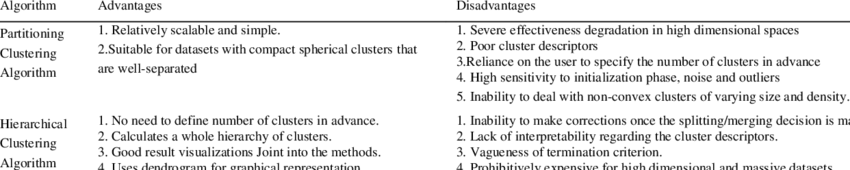
\includegraphics[scale=0.60,center]{Expt8OP/advDisadvClustering.png}
    	\caption{Pros and cons of clustering.}
    	\label{fig:1}
    \end{figure}
\end{enumerate}

\pagebreak
\section{Tools and Packages}
\begin{enumerate}
	\item Tools
	\begin{itemize}
		\item RStudio.
		\item R Version 1.1.463
	\end{itemize}
	\item Clustering and other Packages:
	\begin{itemize}
		\item cluster
		\item factoextra (Visualisation)
		\item magrittr (pipe operator in R)
		\item USArrests Dataset 
	\end{itemize}				
\end{enumerate}

\section{Dataset Description - USArrests}
\begin{itemize}
	\item This data set contains statistics, in arrests per 100,000 residents for assault, murder, and rape in each of the 50 US states in 1973. Also given is the percent of the population living in urban areas. 
	
	\item USArrests is a data frame with :
	\begin{itemize}
		\item 50 observations(rows).
		\item 4 features/variables(columns):
		\begin{itemize}
			\item Murder :  numeric, Murder arrests (per 100,000).
			\item Assault:  numeric, Assault arrests (per 100,000).
			\item UrbanPop: numeric, Percent urban population(per 100,000).
			\item Rape    : numeric, Rape arrests (per 100,000). 
		\end{itemize}
	\end{itemize} 	
\end{itemize}
\section{Procedure}

\begin{enumerate}

	\item Data preparation:
	\begin{itemize}
		\item Remove missing and junk values.
		\item Scale the variables to make them equal.
	\end{itemize} 
	
	\item Split the data set as (Optional):
	\begin{itemize}
		\item Training dataset.
		\item Testing dataset.
	\end{itemize}
    \item Implementation of clustering methodologies:
    \begin{itemize}
    	\item Computation  and visualisation of k-means clustering.
    	\item Computation  and visualisation of k-medoids clustering.
    	\item Computation  and visualisation of PAM clustering.
       \item Computation  and visualisation of Hierarchial clustering.	
    \end{itemize}
	\item Enhanced clustering visualisation using factoextra.
	\item Determining optimal number of clusters.
\end{enumerate}	

\section{Clustering Algorithms}

\begin{itemize}
	\item \textbf{The k-Means Algorithm - Introduction}:
	\begin{enumerate}
		\item Split the input as k categories.
		\item Required: A distance measure - Eucilidean distance
		\item Processing : Clustering based on seed point computed by mean average.
	\end{enumerate}
	\pagebreak
    \item  Pseudocode :
    
    \begin{algorithm}
    	\caption{The \textit{k}-Means Algorithm}
    	\algrule
    	\begin{itemize}
    		\Statex \textbullet~\textbf{Initialisation:}
    		\begin{itemize}
    			\item Choose a value for k.
    			\item Choose k random positions in the input space.
    			\item Assign the cluster centres $\mu$\textsubscript{j} to those positions.
    	\end{itemize}
    	\Statex \textbullet~\textbf{Training}
    		
    		     - Repeat
    			\begin{itemize}
                    \item for each datapoint x i :
                    \begin{itemize}
                    \item compute the distance to each cluster centre.
                    \item assign the datapoint to the nearest cluster centre with distance.
    			\end{itemize}
    			\begin{equation}
    				d\textsubscript{i}= min\textsubscript{j}d(x\textsubscript{i},\mu\textsubscript{j}).
    			\end{equation}
    			\item for each cluster centre :
    			\begin{itemize}
                      \item move the position of the centre to the mean of the points in that cluster
                      (N\textsubscript{j} is the number of points in cluster j):
                      \begin{equation}
                      \mu\textsubscript{j}=\frac{1}{N\textsubscript{j}}\sum_{i=1}^{N\textsubscript{j}}x\textsubscript{i}
                      \end{equation}

    			\end{itemize}
    		\end{itemize}
    	 - until the cluster centres stop moving     
    	\Statex \textbullet~\textbf{Usage}
    	\begin{itemize}
    		\item for each test point :	
    		\begin{itemize}
    			\item Compute the distance to each cluster centre.
    			\item Assign the datapoint to the nearest cluster centre with distance.
    			\begin{equation}
                     d\textsubscript{i}= min\textsubscript{j}d(x\textsubscript{i},\mu\textsubscript{j}).
    			\end{equation}
    		\end{itemize}
    	\end{itemize}		
    		\algrule
    \end{itemize}
    \end{algorithm}
\item \textbf{K-medoids Algorithm - Introduction}:
\begin{enumerate}
        \item K-means is sensitive to outliers and compute large distance.
        \item Change in distance measure as follows :
        \begin{itemize}
        	\item Given ${x={x\textsubscript{1}, x\textsubscript{2},\dots, x\textsubscript{N}}}$
        	\item $ median(x) \in \argmin\textsubscript{z}\sum_{i=1}^{N}|x\textsubscript{i}-z|$
        	\item so could cluster by using the median to construct distance measure.
        	More generally, we can assign cluster “center” to be the cluster medoid so we set m\textsubscript{k}:= x\textsubscript{i\textsubscript{k}} where

        	\begin{equation*}
                 i\textsubscript{k} = \argmin\textsubscript{l} \sum_{i \in C\textsubscript{k}}^{ } d(x\textsubscript{l}, x\textsubscript{i}).
                 where \
                 l \in C\textsubscript{k}
        	\end{equation*}
        	 \end{itemize}
        \item Form new clusters by assigning points to the nearest cluster center.
        \begin{equation*}
           C(i) = \argmin\textsubscript{limit} d(x\textsubscript{i} , m\textsubscript{k})
           where \
            limit - 1\le k \le K
        \end{equation*}
\end{enumerate}
	\pagebreak
	\begin{itemize}
	
	\item  Pseudocode :
	\begin{algorithm}
		\caption{The \textit{k}-Medoids Clustering}
		\algrule
		\begin{itemize}
			\Statex \textbullet~\textbf{Algorithm :}
			\begin{enumerate}
				\item For a given cluster assignment C find the observation in the cluster minimizing total distance to other points in that cluster.
				\begin{equation}
				i\textsubscript{k} = \argmin\textsubscript{l} \sum_{i \in C\textsubscript{k}}^{ } D(x\textsubscript{i}, x\textsubscript{i\textsuperscript{'}}).
				\end{equation}
				where,
				$l \in C\textsubscript{k} , m\textsubscript{k}:= x\textsubscript{i\textsubscript{k}}$ 
				are the current estimates of the cluster centres.	
				
				\item Given a current set of cluster centers = {m\textsubscript{1},\dots,m\textsubscript{K}} minimize the total error by assigning each observation to the closest (current) cluster center:
				 \begin{equation}
				 C(i) = \argmin\textsubscript{limit} d(x\textsubscript{i} , m\textsubscript{k})
				 where \
				 limit - 1\le k \le K
				 \end{equation}
				\item Repeat step 1 and 2 until no change in assignment.
			\end{enumerate}
			\algrule
		\end{itemize}
		\end{algorithm}
\end{itemize}
\item \textbf{Hierarcial clustering- Introduction}:
\begin{enumerate}
	\item Clusters at a given level are created by merging clusters at the next lower level.
	\item Each cluster at the lowest level contains a single observation.
	\item At the highest level there is just one cluster containing all the data.
	\item There are two basic paradigms for constructing hierarchical clusters
	\begin{itemize}
         \item Agglomerative : bottom-up
         \item Divisive : top-down
	\end{itemize}
\end{enumerate}
\item Pseudocode :
\begin{algorithm}
	\caption{Hierarcial clustering}
	\algrule
	\begin{itemize}
		\Statex \textbullet~\textbf{Algorithm :}
		\begin{enumerate}
			\item Begin with the disjoint clustering having level L(0) = 0 and sequence number m = 0.
			\item Find the least dissimilar pair of clusters in the current clustering, say pair (r), (s), according to.
			\begin{equation}
			d[(r),(s)] = min d[(i),(j)]
			\end{equation}
			\textit{where the minimum is over all pairs of clusters in the current clustering.
			}
			\item Increment the sequence number : m = m +1. Merge clusters (r) and (s) into a single cluster to form the next clustering m. Set the level of this clustering to
			\begin{equation}
		     L(m) = d[(r),(s)]
			\end{equation}
			\item Update the proximity matrix, D, by deleting the rows and columns corresponding to clusters (r) and (s) and adding a row and column corresponding to the newly formed cluster. The proximity between the new cluster, denoted (r,s) and old cluster (k) is defined in this way:
			\begin{equation}
			d[(k), (r,s)] = min d[(k),(r)], d[(k),(s)]
			\end{equation}
			\item If all objects are in one cluster, stop. Else, go to step 2.
			
		\end{enumerate}
		\algrule
	\end{itemize}
\end{algorithm}
\end{itemize}

\newpage
\section{Confusion Matrix}
\begin{itemize}
\item A confusion matrix is a table that can be generated for a classifier on a Data Set 

\textbf{True Positives(TP)-} These are the cases where the predicted and actual both are yes.
\linebreak
\textbf{True Negatives(TN)-} These are the cases where the predicted value is no and actual value is yes.
\linebreak
\textbf{False Positive(FP)-} These are the cases where the predicted value is yes and actual value is no.
\linebreak
\textbf{False Negative(FN)-} These are the cases where prediction is no and actual value is no.
\end{itemize}


\section{Coding}

\lstinputlisting{clustering.R}
\newpage
\section{Output} 
\verbatiminput{clusteringOutput.txt}
\fbox{\begin{minipage}{35em}
		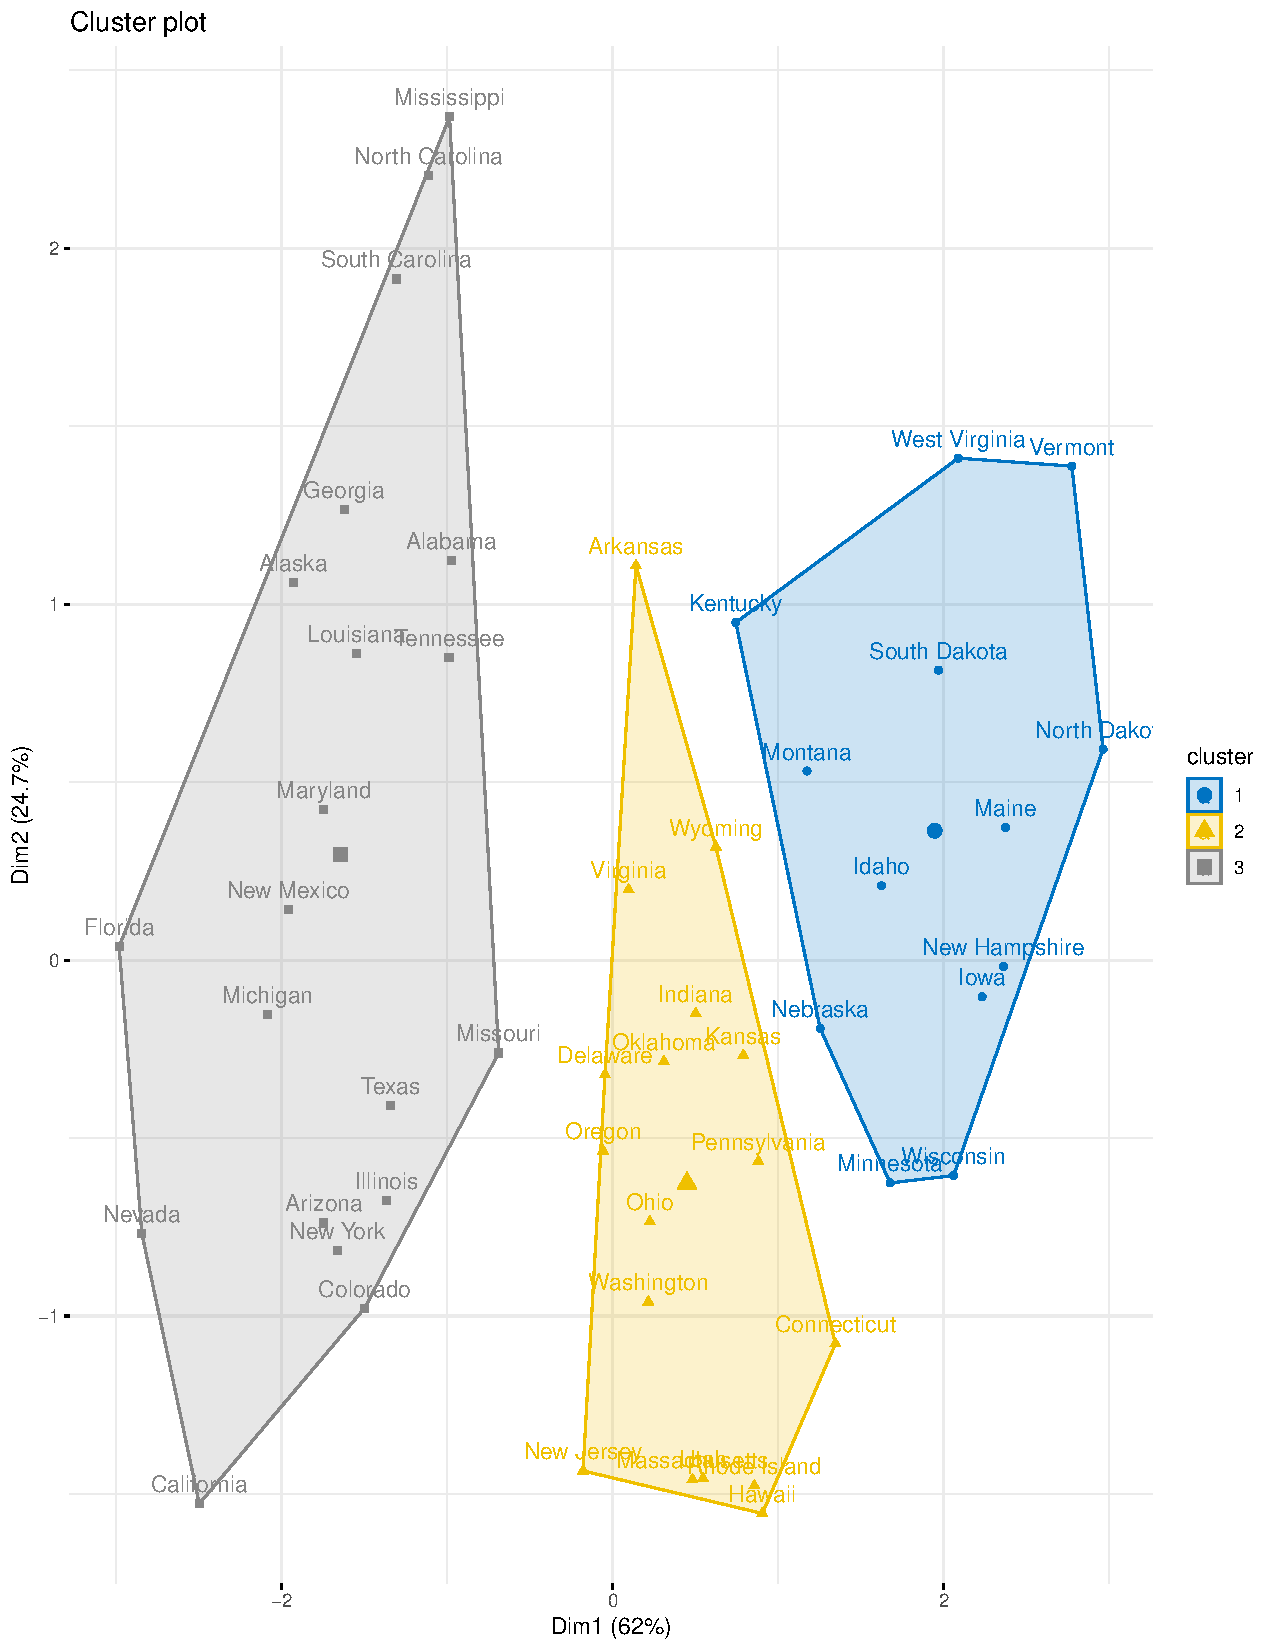
\includegraphics[page=1,scale=0.4]{Expt8OP/clusterPlot.pdf}
	\end{minipage}}

\fbox{\begin{minipage}{35em}
		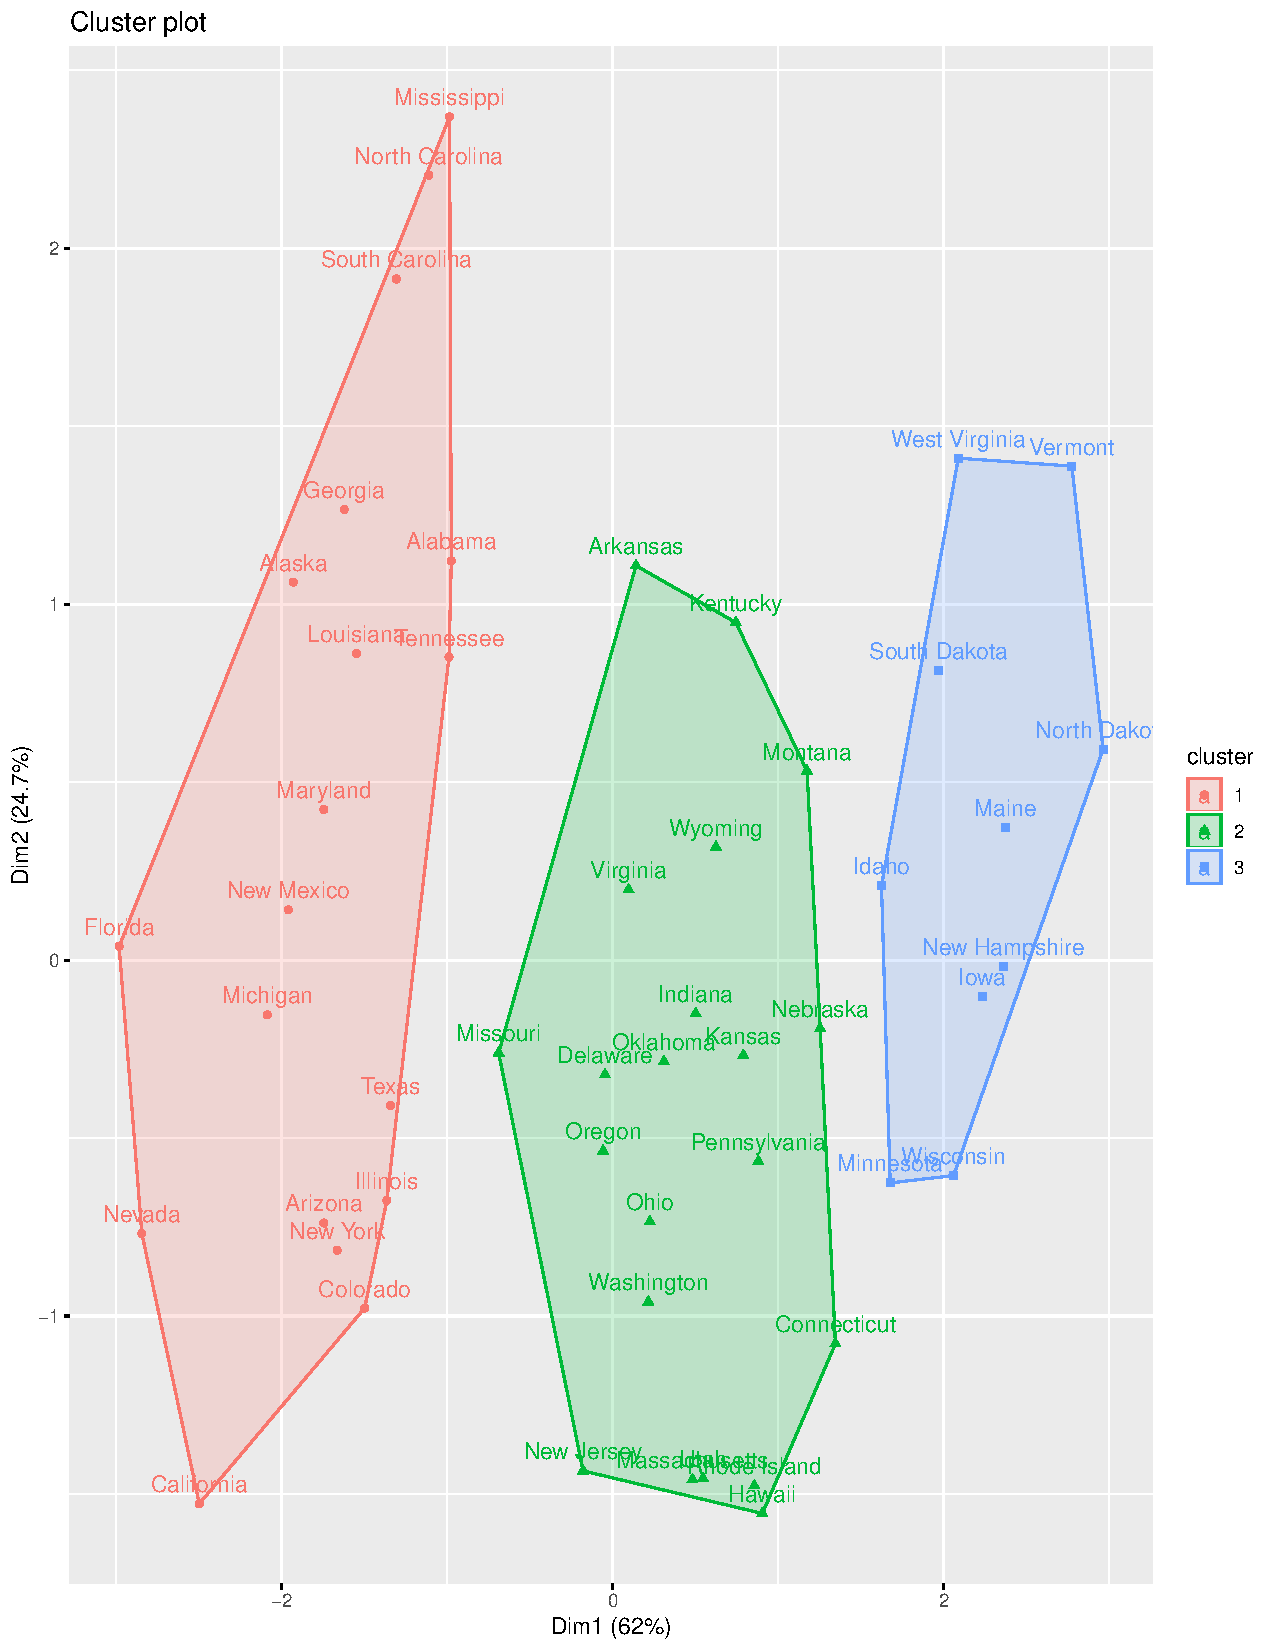
\includegraphics[page=1,scale=0.4]{Expt8OP/clusterPlotTwo.pdf}
\end{minipage}}

\fbox{\begin{minipage}{35em}
		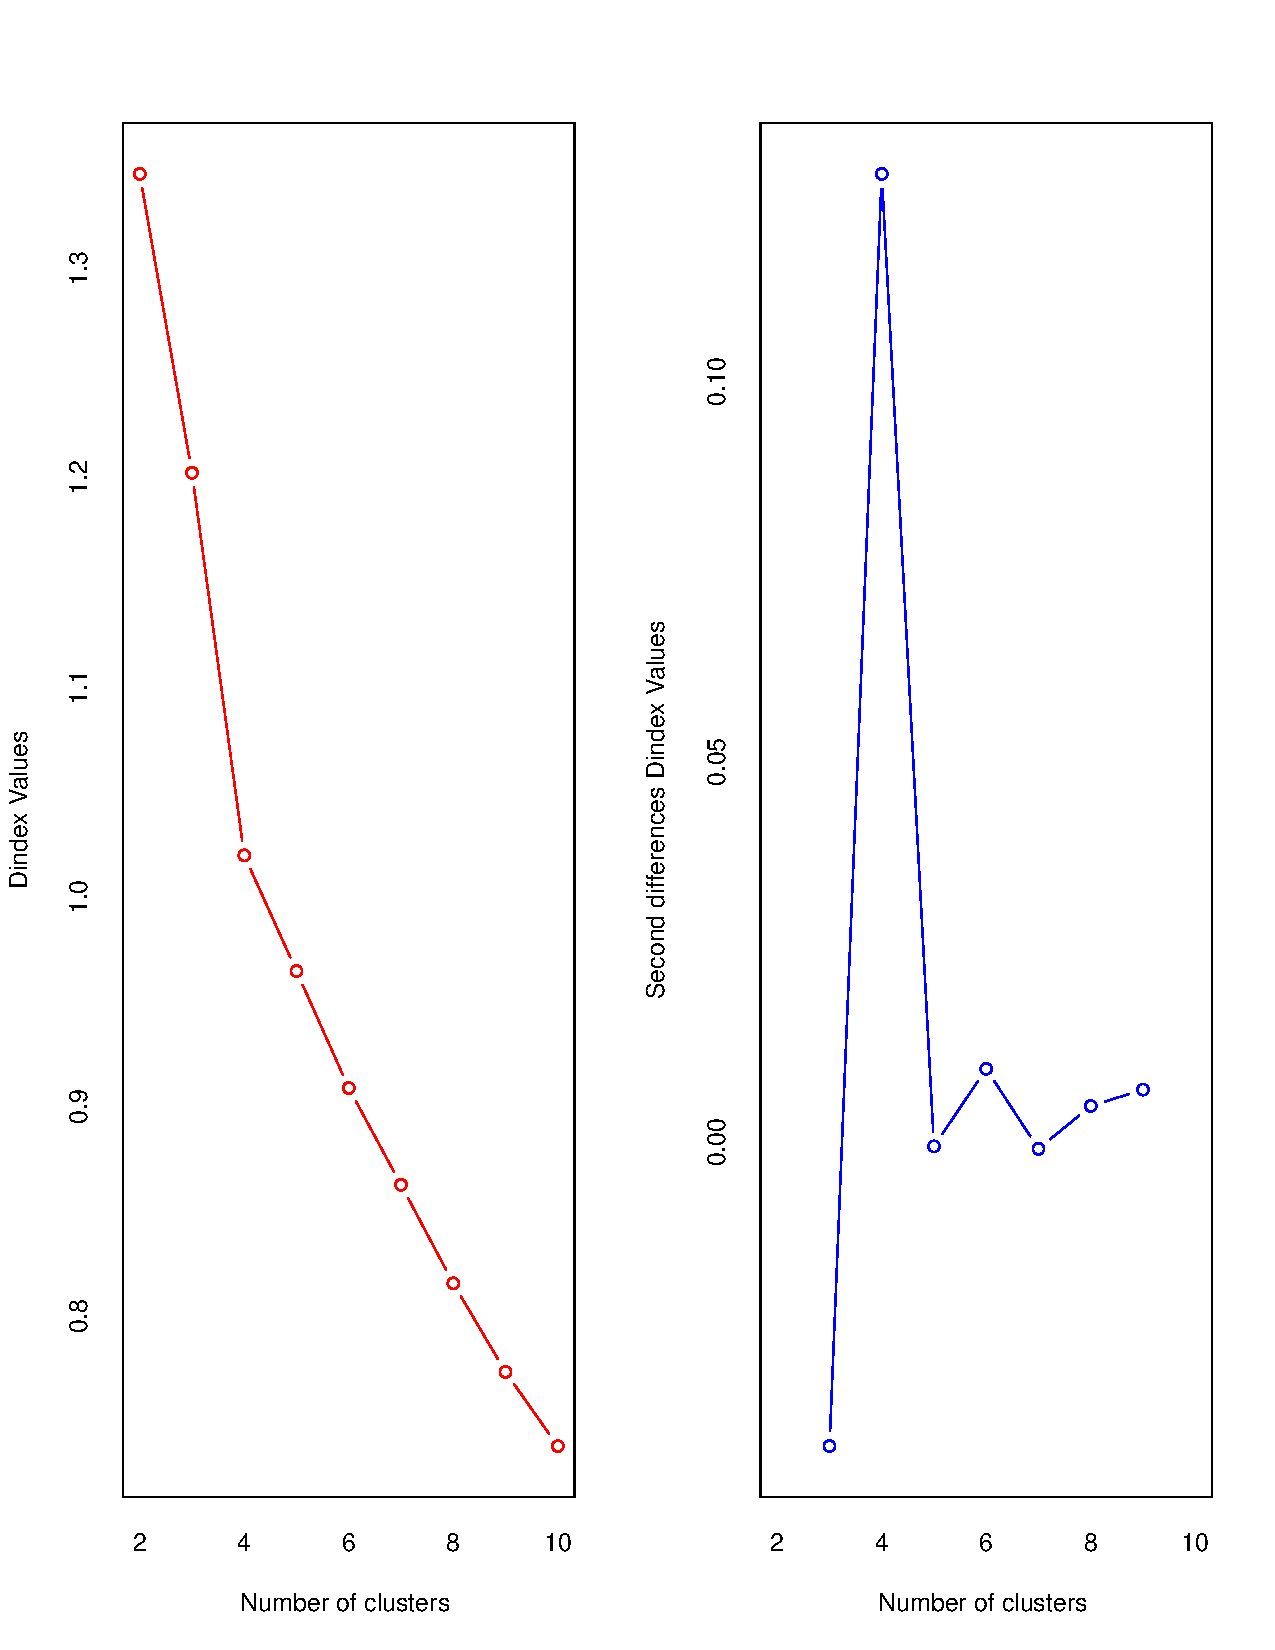
\includegraphics[page=1,scale=0.4,angle=270]{Expt8OP/DindexValues.pdf}
\end{minipage}}

\fbox{\begin{minipage}{35em}
		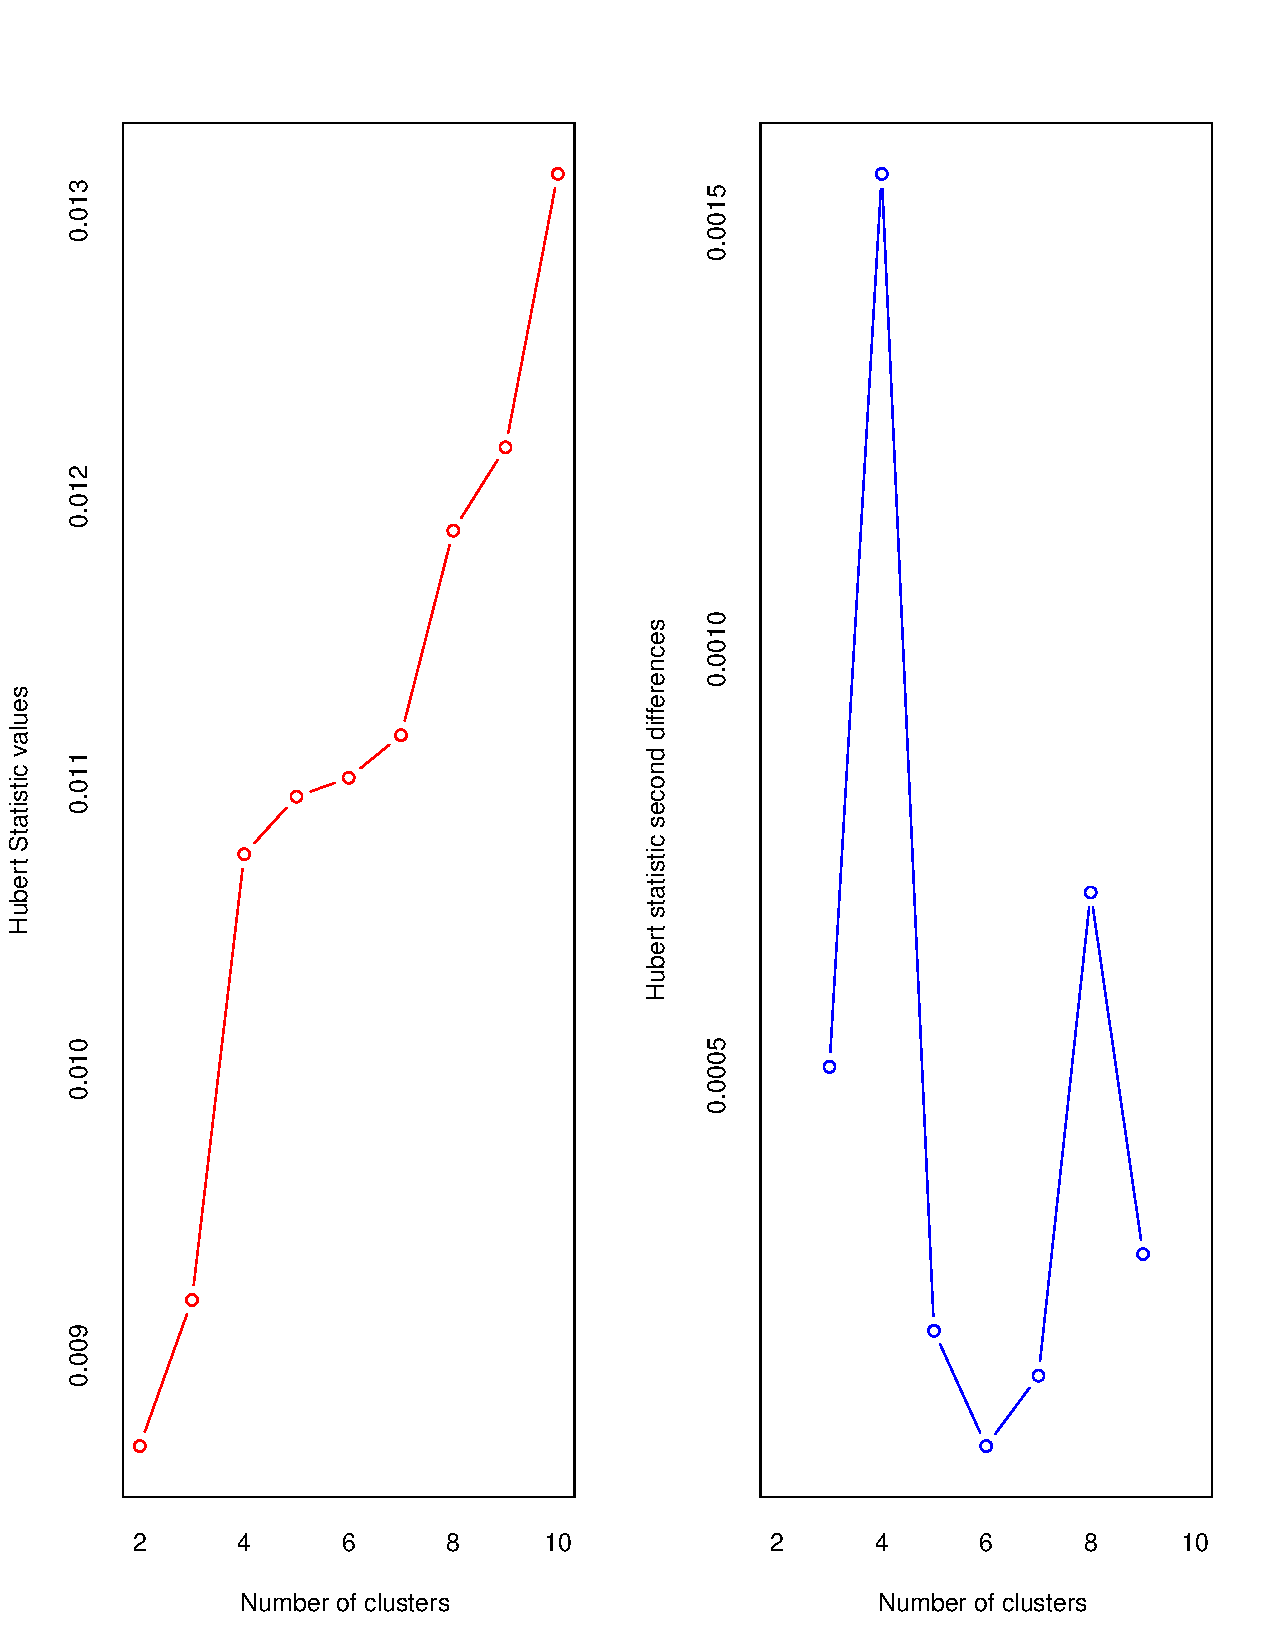
\includegraphics[page=1,scale=0.4,angle=270]{Expt8OP/hubertStatisticValues.pdf}
\end{minipage}}

\fbox{\begin{minipage}{35em}
		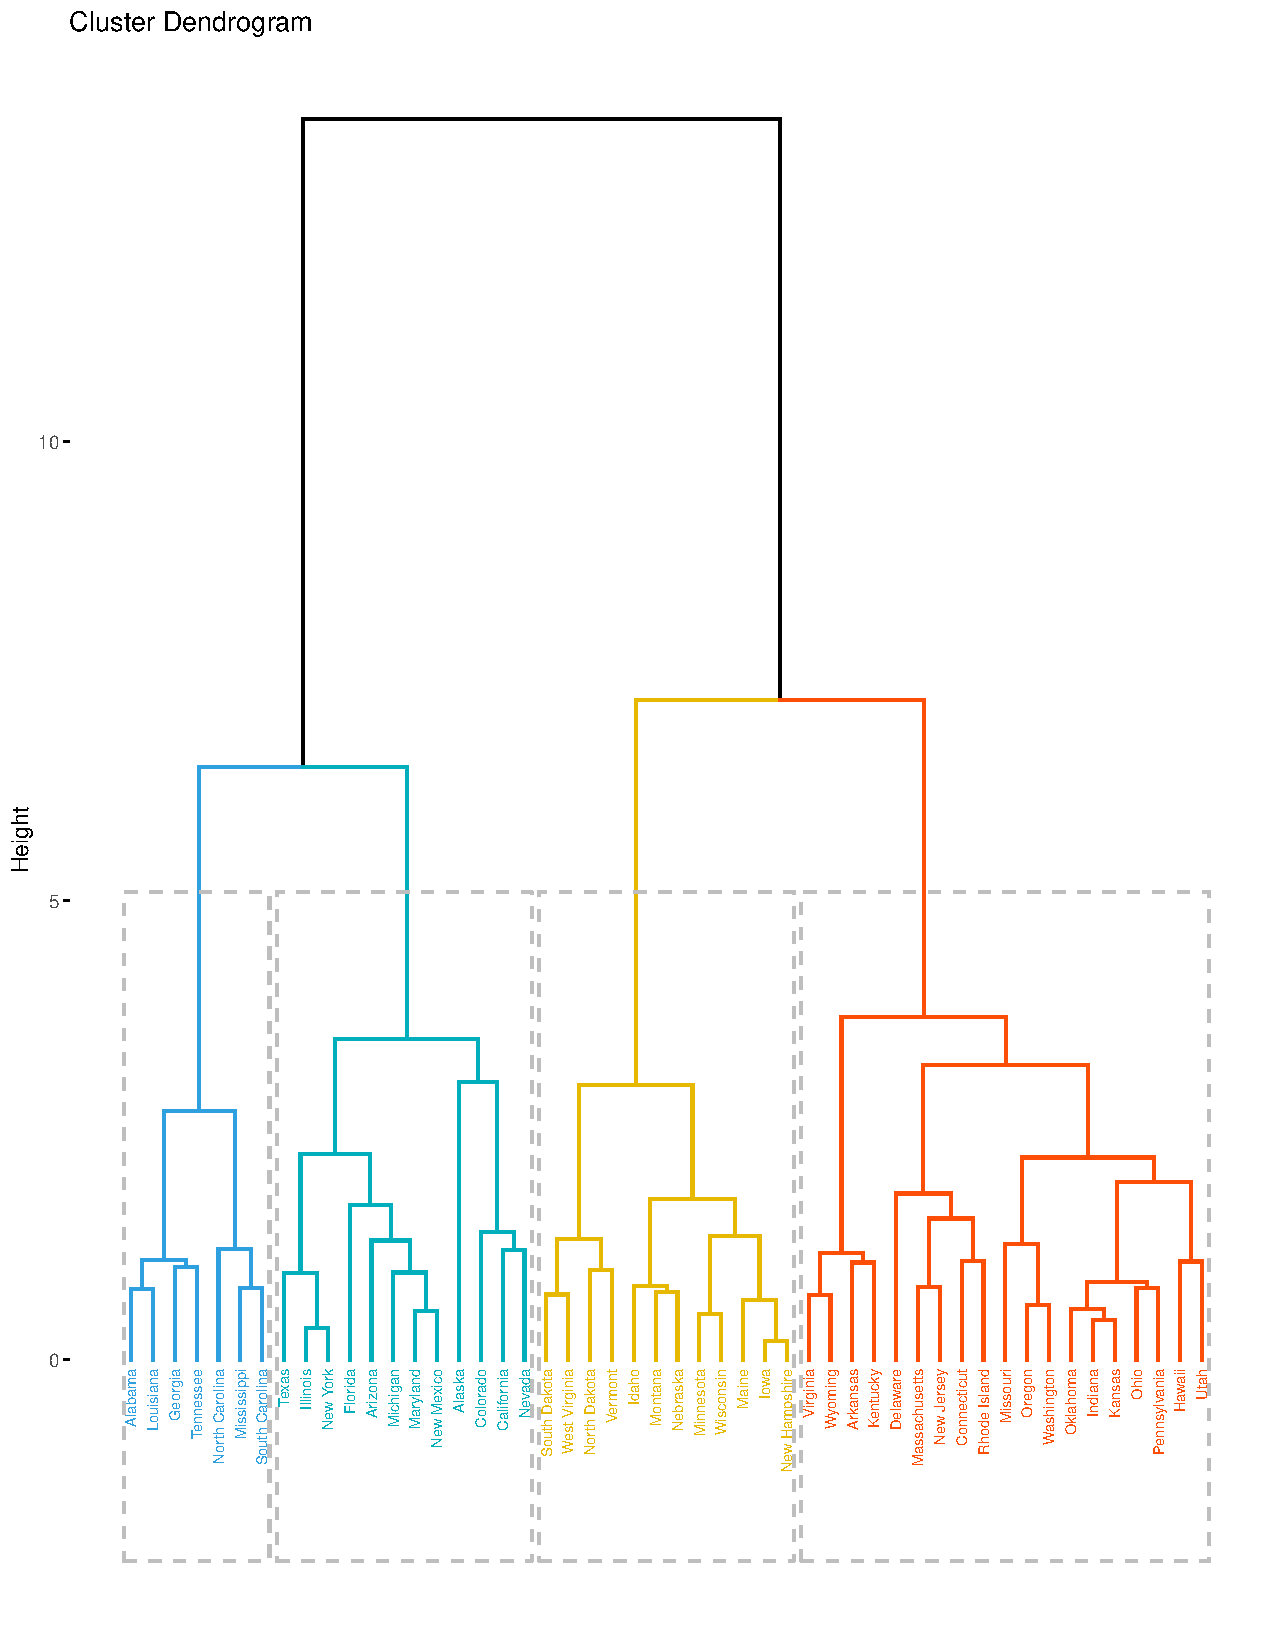
\includegraphics[page=1,scale=0.5]{Expt8OP/clusterDendrogram.pdf}
\end{minipage}}


\fbox{\begin{minipage}{35em}
		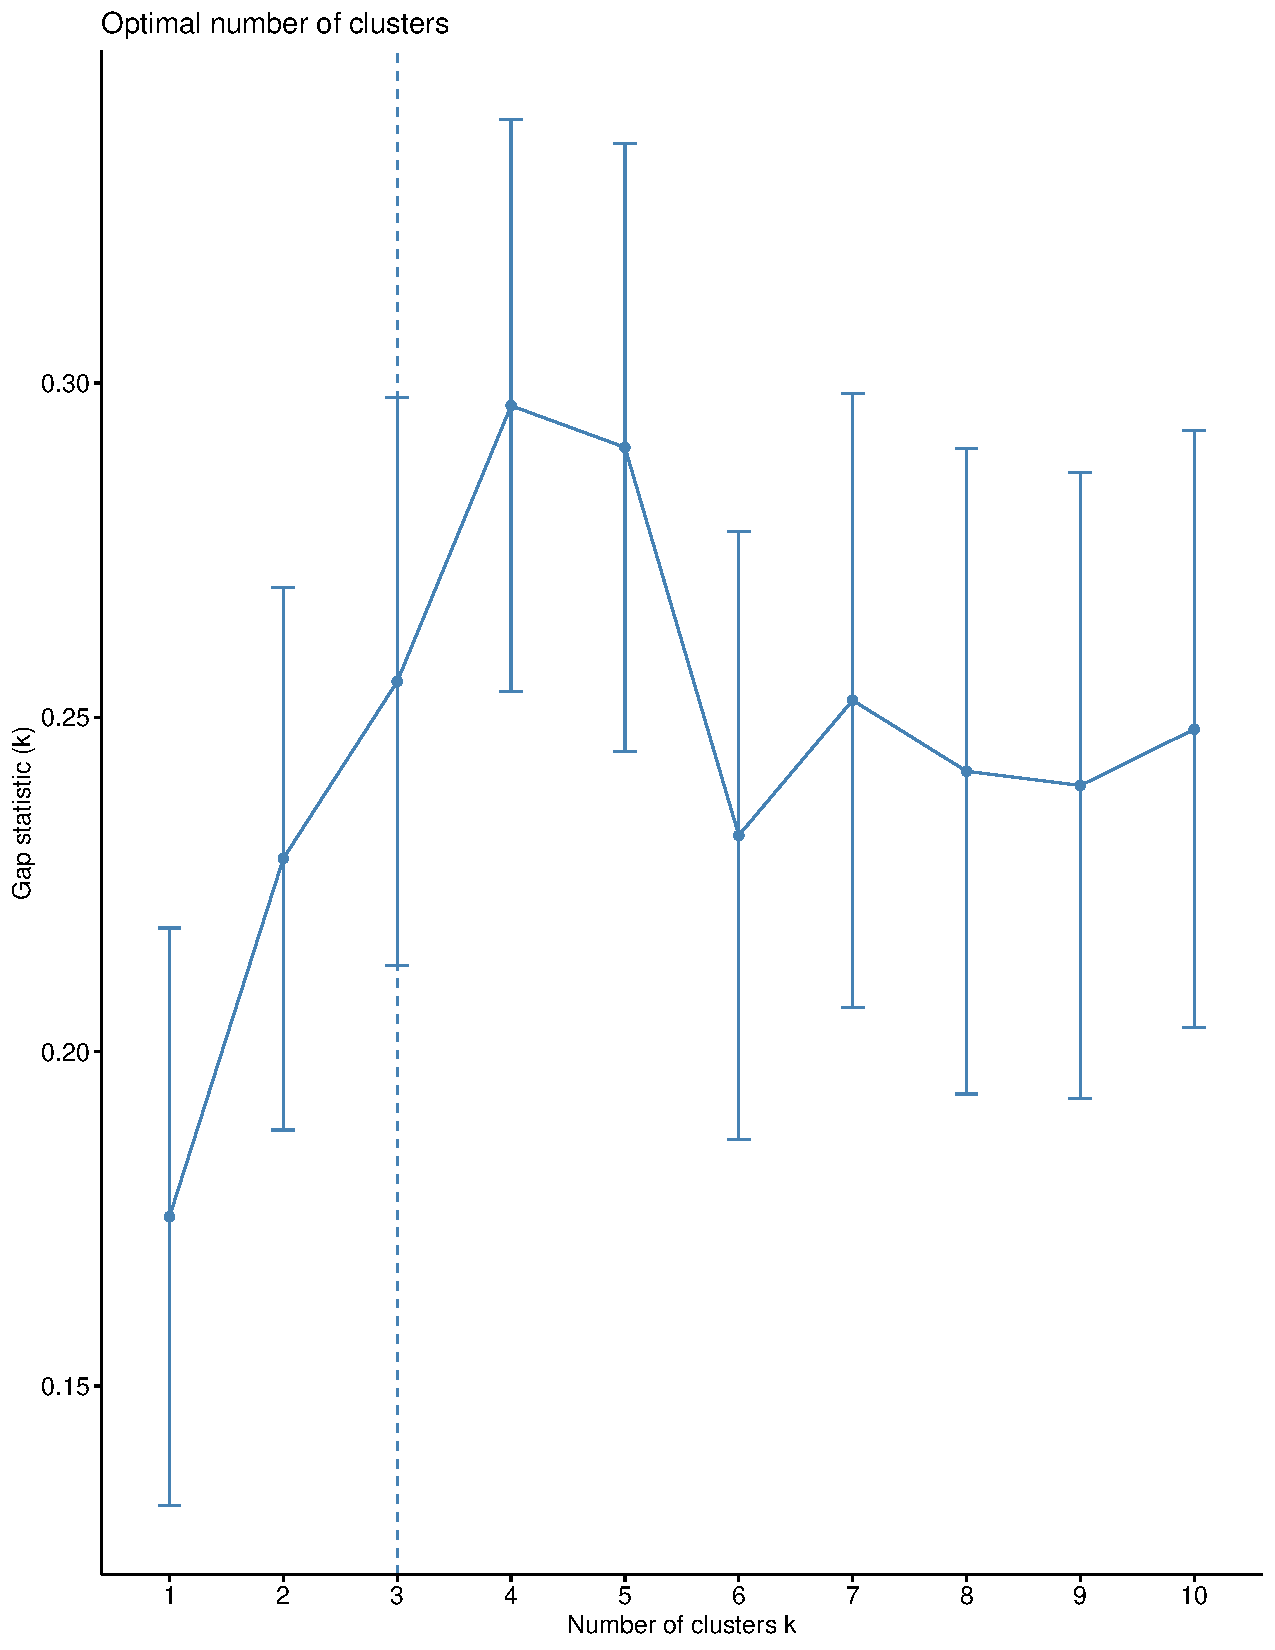
\includegraphics[page=1,scale=0.4]{Expt8OP/OptimalNoOfClusters.pdf}
\end{minipage}}
\linebreak
\linebreak
\vfill
\section{Result}
Thus the implementation of clustering is executed successfully using R program on USArrests Dataset.
\end{document}